\documentclass{standalone}
% ------------------------------------------------------------------------------
% Packages
% ------------------------------------------------------------------------------
\usepackage[ddmmyyyy]{datetime}
\usepackage[T1]{fontenc}
\usepackage[utf8]{inputenc}

% Page setting
\usepackage[explicit]{titlesec}
\usepackage{sectsty}
\usepackage{fancyhdr}
\usepackage[title, titletoc]{appendix}

% Fonts
\usepackage{kpfonts}
\usepackage{amsmath}
\usepackage{amssymb}
\usepackage{dsfont}
\usepackage{pifont}

% Graphics and colors
\usepackage{graphicx}
\usepackage{xcolor}
\usepackage{import}

\definecolor{myred}{RGB}{150,0,0}
\definecolor{mygreen}{RGB}{0,150,0}
\definecolor{myblue}{RGB}{0, 101, 189}
\definecolor{myyellow}{RGB}{220, 206, 0}
\definecolor{myorange}{RGB}{255, 153, 51}
\definecolor{mycyan}{RGB}{51, 204, 204}
\definecolor{mypurple}{RGB}{204, 0, 153}

\newcommand{\doccol}{\color{myblue}}

% Hyperrefs
\usepackage[
  pdfusetitle,
  unicode = true,
  bookmarks = true,
  bookmarksnumbered = false,
  bookmarksopen = true,
  breaklinks = false,
  pdfborderstyle = {},
  backref = false,
  colorlinks = true,
  linkcolor = myblue,
  urlcolor = myred,
  citecolor = mygreen,
]{hyperref}


% Captions
\usepackage{caption}

\captionsetup[figure]{position = bottom}
\captionsetup[table]{position = bottom}

% Tables, Algs ...
\usepackage{enumitem}
\usepackage{algorithm}
\usepackage{algorithmicx}
\usepackage{algpseudocode}
\usepackage{booktabs}
\usepackage{nicematrix}

\renewcommand{\arraystretch}{1.5}

\newcommand{\headercol}{myblue!20}
\newcommand{\rowcol}{myblue!10}

% Math
\usepackage{nicefrac}
\usepackage{bm}
\usepackage{thm-restate}
\usepackage{optidef}
\usepackage{xspace}

% Theorems
\usepackage[framemethod=TikZ]{mdframed}
\usepackage{amsthm}
\usepackage{xifthen}

% Tikz and pfgplots
\usepackage{tikz}
\usepackage{pgfplots}
\usepackage{pgfplotstable}

\usetikzlibrary{shapes}
\usetikzlibrary{arrows}
\usetikzlibrary{automata}
\usetikzlibrary{positioning}
\usetikzlibrary{calc}
\usetikzlibrary{intersections}

\pgfplotsset{compat=newest}
\usepgfplotslibrary{groupplots}
\usepgfplotslibrary{fillbetween}

\tikzstyle{line_node} = [line width=1pt, rounded corners, color=black, ->]
\tikzstyle{line_cv} = [line width=3pt, color=mygreen, line cap=round]

% Tmp
\usepackage[color=myred!50]{todonotes}

% ------------------------------------------------------------------------------
% Math declarations
% ------------------------------------------------------------------------------
\newcommand{\Brac}[2][r]{%
  \ifx r#1 \left(       #2 \right)       \else
  \ifx c#1 \left\{      #2 \right\}      \else
  \ifx s#1 \left[       #2 \right]       \else
  \ifx v#1 \left\vert   #2 \right\vert   \else
  \ifx a#1 \left\langle #2 \right\rangle \else
  \ifx t#1 \left\lceil  #2 \right\rceil  \else
  \ifx b#1 \left\lfloor #2 \right\rfloor \else
  \ifx n#1 \left\|      #2 \right\|      \else
  \mathrm{Illegal~option}%
  \fi\fi\fi\fi\fi\fi\fi\fi
}

\newcommand{\clip}[4][s]{
  \ifx s#1 \mathrm{clip}_{\Brac[s]{#2,\; #3}}\Brac{#4} \else
  \ifx u#1 \mathrm{clip}_{\left[#2,\; #3\right)}\Brac{#4} \else
  \ifx l#1 \mathrm{clip}_{\left(#2,\; #3\right]}\Brac{#4} \else
  \mathrm{Illegal~option}%
  \fi\fi\fi
}

\DeclareMathOperator*{\argmax}{arg\,max}

\newcommand{\yesmark}{\textcolor{mygreen}{\ding{51}}}%
\newcommand{\nomark}{\textcolor{myred}{\ding{55}}}
\newcommand{\good}[1]{\textcolor{mygreen}{#1}}
\newcommand{\bad}[1]{\textcolor{myred}{#1}}

\newcommand{\R}{\mathbb{R}}
\newcommand{\N}{\mathbb{N}}
\newcommand{\X}{\mathbb{X}}

\newcommand{\I}{\mathcal{I}}
\newcommand{\Itil}{\tilde{\mathcal{I}}}
\newcommand{\Ineg}{\I_{-}}
\newcommand{\Ipos}{\I_{+}}

\newcommand{\Imb}{\I_{\text{mb}}}
\newcommand{\Imbneg}{\I_{\text{mb},-}}
\newcommand{\Imbpos}{\I_{\text{mb},+}}

\newcommand{\indmax}{j^{\star}}
\newcommand{\indmaxmb}{j^{\star}_{\text{mb}}}

\newcommand{\nall}{n}
\newcommand{\nneg}{n_{-}}
\newcommand{\npos}{n_{+}}
\newcommand{\ntil}{\tilde{n}}

\newcommand{\nmb}{n_{\text{mb}}}
\newcommand{\nmbneg}{n_{\text{mb},-}}
\newcommand{\nmbpos}{n_{\text{mb},+}}

\newcommand{\K}{\mathbb{K}}
\newcommand{\Kall}{\K^{\pm}}
\newcommand{\Kneg}{\K^{-}}

\newcommand{\alphak}{\alpha_{\hat{k}}}
\newcommand{\alphal}{\alpha_{\hat{l}}}
\newcommand{\betak}{\beta_{\hat{k}}}
\newcommand{\betal}{\beta_{\hat{l}}}

\newcommand{\norm}[1]{\Brac[n]{#1}}
\newcommand{\abs}[1]{|#1|}
\newcommand{\inner}[2]{\Brac[a]{#1, \; #2}}
\newcommand{\dd}[1]{\mathop{}\!\mathrm{d}#1}

\newcommand{\Iverson}[1]{\mathds{1}_{\Brac[s]{#1}}}

\newcommand{\EE}{\mathbb{E}}
\newcommand{\PP}{\mathbb{P}}
\newcommand{\bias}{\operatorname{bias}}

\newcommand{\Matrix}[1]{\begin{pmatrix} #1 \end{pmatrix}}
\newcommand{\Set}[2]{\Brac[c]{#1 \; \middle\vert \; #2}}
\newcommand{\domain}{\operatorname*{dom}}

\newcommand{\repeatloop}{\texttt{repeat}\xspace}
\newcommand{\forloop}{\texttt{for}\xspace}

\newcommand{\vecab}{\Matrix{\bm{\alpha} \\ \bm{\beta}}}

% models
\newcommand{\AccatTop}{\emph{Accuracy at the Top}\xspace}
\newcommand{\TopPush}{\emph{TopPush}\xspace}
\newcommand{\TopPushK}{\emph{TopPushK}\xspace}
\newcommand{\tauFPL}{{\emph{$\tau$-FPL}}\xspace}
\newcommand{\TopMeanK}{\emph{TopMeanK}\xspace}
\newcommand{\PatMat}{\emph{Pat}\&\emph{Mat}\xspace}
\newcommand{\PatMatNP}{{\emph{Pat}\&\emph{Mat-NP}}\xspace}
\newcommand{\Grill}{\emph{Grill}\xspace}
\newcommand{\GrillNP}{\emph{Grill-NP}\xspace}
\newcommand{\DeepTopPush}{\emph{DeepTopPush}\xspace}
\newcommand{\TFCO}{\emph{TFCO}\xspace}
\newcommand{\APPerf}{\emph{Ap-Perf}\xspace}
\newcommand{\BaseLine}{\emph{BinCross}\xspace}
\newcommand{\SVM}{\emph{SVM}\xspace}

% counts and rates
\DeclareMathOperator{\tp}{tp}
\DeclareMathOperator{\tn}{tn}
\DeclareMathOperator{\fp}{fp}
\DeclareMathOperator{\fn}{fn}
\DeclareMathOperator{\tpr}{tpr}
\DeclareMathOperator{\tnr}{tnr}
\DeclareMathOperator{\fpr}{fpr}
\DeclareMathOperator{\fnr}{fnr}

\DeclareMathOperator{\tps}{\overline{tp}}
\DeclareMathOperator{\tns}{\overline{tn}}
\DeclareMathOperator{\fps}{\overline{fp}}
\DeclareMathOperator{\fns}{\overline{fn}}

\DeclareMathOperator{\accuracy}{acc}
\DeclareMathOperator{\baccuracy}{bacc}
\DeclareMathOperator{\precision}{precision}
\DeclareMathOperator{\recall}{recall}
\DeclareMathOperator{\pratrec}{Precision@Recall}
\DeclareMathOperator{\postop}{pos@top}

\newcommand{\tpratk}{\operatorname{TPR@}K}
\newcommand{\tpratfpr}{\operatorname{TPR@}\tau}
\newcommand{\auroc}{\operatorname{AUROC}}


% ------------------------------------------------------------------------------
% Document
% ------------------------------------------------------------------------------
\tikzstyle{critline1} = [
  line width=1pt,
  rounded corners,
  color=black,
  ->,
]
\tikzstyle{critline2} = [
  line width=3pt,
  color=mygreen,
  line cap=round,
]

\begin{document}
% 
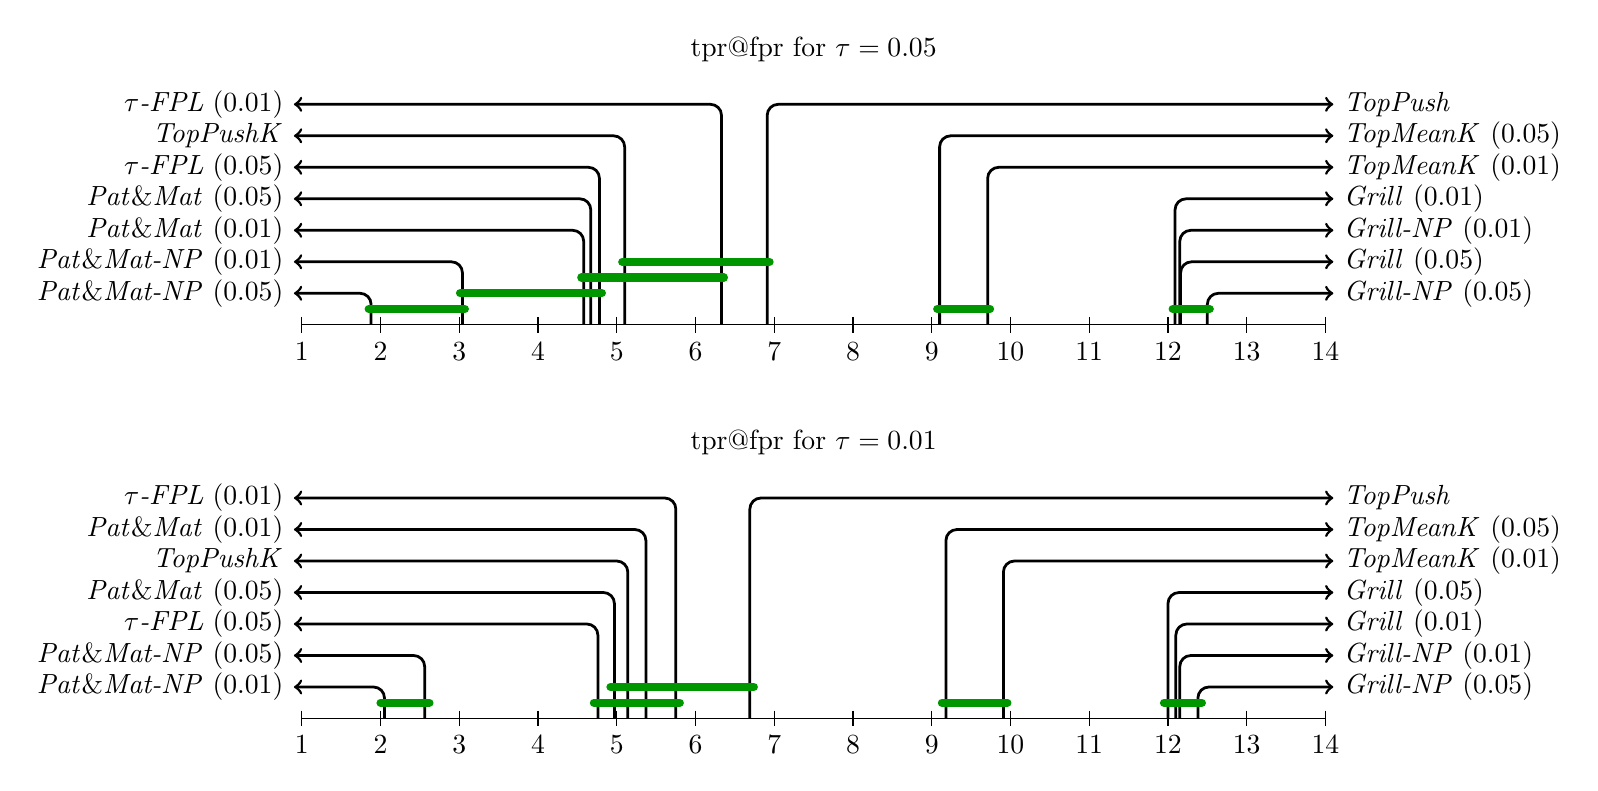
\begin{tikzpicture}
  \node at (7.5,3.5) {tpr@fpr for $\tau = 0.01$};
  \draw (1.0,0)--(14.0,0);
  \foreach \x in {1,...,14} \draw (\x,0.10)--(\x,-0.10) node[anchor=north]{$\x$};
  \draw[critline1] (2.05,0)--(2.05,0.4)--(0.9,0.4) node[anchor=east] {\PatMatNP(0.01)};
  \draw[critline1] (2.56,0)--(2.56,0.8)--(0.9,0.8) node[anchor=east] {\PatMatNP(0.05)};
  \draw[critline1] (4.76,0)--(4.76,1.2)--(0.9,1.2) node[anchor=east] {\tauFPL(0.05)};
  \draw[critline1] (4.97,0)--(4.97,1.6)--(0.9,1.6) node[anchor=east] {\PatMat(0.05)};
  \draw[critline1] (5.14,0)--(5.14,2.0)--(0.9,2.0) node[anchor=east] {\TopPushK};
  \draw[critline1] (5.37,0)--(5.37,2.4)--(0.9,2.4) node[anchor=east] {\PatMat(0.01)};
  \draw[critline1] (5.75,0)--(5.75,2.8)--(0.9,2.8) node[anchor=east] {\tauFPL(0.01)};
  \draw[critline1] (6.69,0)--(6.69,2.8)--(14.1,2.8) node[anchor=west] {\TopPush};
  \draw[critline1] (9.18,0)--(9.18,2.4)--(14.1,2.4) node[anchor=west] {\TopMeanK(0.05)};
  \draw[critline1] (9.91,0)--(9.91,2.0)--(14.1,2.0) node[anchor=west] {\TopMeanK(0.01)};
  \draw[critline1] (12,0)--(12,1.6)--(14.1,1.6) node[anchor=west] {\Grill(0.05)};
  \draw[critline1] (12.1,0)--(12.1,1.2)--(14.1,1.2) node[anchor=west] {\Grill(0.01)};
  \draw[critline1] (12.15,0)--(12.15,0.8)--(14.1,0.8) node[anchor=west] {\GrillNP(0.01)};
  \draw[critline1] (12.38,0)--(12.38,0.4)--(14.1,0.4) node[anchor=west] {\GrillNP(0.05)};

  \draw[critline2] (2.00,0.2)--(2.62,0.2);
  \draw[critline2] (4.71,0.2)--(5.80,0.2);
  \draw[critline2] (4.92,0.4)--(6.74,0.4);
  \draw[critline2] (9.13,0.2)--(9.96,0.2);
  \draw[critline2] (11.95,0.2)--(12.43,0.2);

  \node at (7.5,8.5) {tpr@fpr for $\tau = 0.05$};
  \draw (1.0,5)--(14.0,5);
  \foreach \x in {1,...,14} \draw (\x,5.10)--(\x,4.90) node[anchor=north]{$\x$};
  \draw[critline1] (1.88,5.0)--(1.88,5.4)--(0.9,5.4) node[anchor=east] {\PatMatNP(0.05)};
  \draw[critline1] (3.04,5.0)--(3.04,5.8)--(0.9,5.8) node[anchor=east] {\PatMatNP(0.01)};
  \draw[critline1] (4.58,5.0)--(4.58,6.2)--(0.9,6.2) node[anchor=east] {\PatMat(0.01)};
  \draw[critline1] (4.67,5.0)--(4.67,6.6)--(0.9,6.6) node[anchor=east] {\PatMat(0.05)};
  \draw[critline1] (4.78,5.0)--(4.78,7.0)--(0.9,7.0) node[anchor=east] {\tauFPL(0.05)};
  \draw[critline1] (5.1,5.0)--(5.1,7.4)--(0.9,7.4) node[anchor=east] {\TopPushK};
  \draw[critline1] (6.33,5.0)--(6.33,7.8)--(0.9,7.8) node[anchor=east] {\tauFPL(0.01)};
  \draw[critline1] (6.91,5.0)--(6.91,7.8)--(14.1,7.8) node[anchor=west] {\TopPush};
  \draw[critline1] (9.1,5.0)--(9.1,7.4)--(14.1,7.4) node[anchor=west] {\TopMeanK(0.05)};
  \draw[critline1] (9.71,5.0)--(9.71,7.0)--(14.1,7.0) node[anchor=west] {\TopMeanK(0.01)};
  \draw[critline1] (12.09,5.0)--(12.09,6.6)--(14.1,6.6) node[anchor=west] {\Grill(0.01)};
  \draw[critline1] (12.15,5.0)--(12.15,6.2)--(14.1,6.2) node[anchor=west] {\GrillNP(0.01)};
  \draw[critline1] (12.16,5.0)--(12.16,5.8)--(14.1,5.8) node[anchor=west] {\Grill(0.05)};
  \draw[critline1] (12.5,5.0)--(12.5,5.4)--(14.1,5.4) node[anchor=west] {\GrillNP(0.05)};
  
  \draw[critline2] (1.85,5.2)--(3.07,5.2);
  \draw[critline2] (3.01,5.4)--(4.81,5.4);
  \draw[critline2] (4.55,5.6)--(6.36,5.6);
  \draw[critline2] (5.07,5.8)--(6.94,5.8);
  \draw[critline2] (9.07,5.2)--(9.74,5.2);
  \draw[critline2] (12.06,5.2)--(12.53,5.2);
\end{tikzpicture}
% 
\end{document}
